% !TEX TS-program = pdflatex
% !TEX encoding = UTF-8 Unicode
\documentclass[12pt,
    driverfallback=dvipdfm,
 %   openright,
 	openany,
    a4paper,
 %   parskip=half,   
    toc=bibliography,
    twoside,
    numbers=noenddot]{article}              % Book class in 11 points

\usepackage[usenames,dvipsnames,showerrors,usenames,svgnames]{xcolor}
    
\usepackage{algorithmic}
\usepackage{fullpage}
\usepackage[hidelinks,breaklinks]{hyperref}
\usepackage[xcolor,makeidx=compatibility,quotation,notion]{knowledge}

\usepackage{float}
\floatstyle{ruled}
\newfloat{problem}{thp}{lop}
\floatname{problem}{Problem}
\usepackage{enumitem}
\usepackage{multicol}
\usepackage[rightcaption]{sidecap}
 
%%% PACKAGES
\usepackage{tikz}
\usetikzlibrary{angles}
\usepackage{graphicx}
\usepackage[export]{adjustbox}


\usepackage[english]{babel}
\usepackage{amsmath, amsthm, amssymb}
%\usepackage{tikz-cd}
%\usetikzlibrary{shapes,arrows,intersections}
%\usetikzlibrary{matrix,fit,calc,trees,positioning,arrows,chains,shapes.geometric,shapes,angles,quotes}

\usepackage{algorithm,algorithmic}% http://ctan.org/pkg/algorithms

\usepackage{mdframed} 
\usepackage{xspace}

\usepackage[capitalize]{cleveref}
\usepackage{todonotes}




\title{\bf $\approxratio$-approximation of MaxCut}    % Supply information
\author{Sreejith A V \footnote{Thanks to Divya Padmanabhan}}              %   for the title page.
\date{}                           %   Use current date.


\newtheorem{theorem}{Theorem}
\newtheorem{corollary}{Corollary}
\newtheorem{definition}{Definition}
\newtheorem{exercise}{Exercise}
\newtheorem{example}{Example}
\newtheorem{puzzle}{Puzzle}
\newtheorem*{solution}{Solution}

\newtheorem{innercustomgeneric}{\customgenericname}
\providecommand{\customgenericname}{}
\newcommand{\newcustomtheorem}[2]{%
  \newenvironment{#1}[1]
  {%
   \renewcommand\customgenericname{#2}%
   \renewcommand\theinnercustomgeneric{##1}%
   \innercustomgeneric
  }
  {\endinnercustomgeneric}
}

\newcustomtheorem{customthm}{Theorem}
\newcustomtheorem{customlemma}{Lemma}
\newtheorem{lemma}[theorem]{Lemma}
\newtheorem{claim}[theorem]{Claim}

\definecolor{light-gray}{gray}{0.95}
\newcommand{\odd}{{\normalfont{Odd}}\xspace}
\newcommand{\even}{{\normalfont{Even}}\xspace}
\newcommand{\finocc}[1]{\mathrm{FIN}(#1)\xspace}
\newcommand{\infocc}[1]{\mathrm{INF}(#1)\xspace}

\newcommand{\Nat}{\mathbb{N}}
\newcommand{\Reals}{\mathbb{R}}
\newcommand{\Rn}{\Reals^n}
\newcommand{\closedset}[2]{[#1, #2]}

\renewcommand{\vec}[1]{\mathbf #1}
\newcommand{\mat}[1]{{\mathbb #1}}
\newcommand{\trans}[1]{{#1}^{\mathsf{T}}}
\newcommand{\rowvec}[1]{\trans{\vec {#1}}}
\newcommand{\dotprod}[2]{\rowvec{#1}  \vec{#2}}
\newcommand{\minimize}{\mathtt{minimize}}
\newcommand{\maximize}{\mathtt{maximize}}

\newcommand{\Imatrix}{\mat{I}}
\newcommand{\cspace}[1]{C(\mat #1)}
\newcommand{\defs}{::=}
\newcommand{\BFS}{\ensuremath{\mathrm{BFS}}\xspace}

\newcommand{\lpstd}[4]{\begin{align*}
\minimize ~\dotprod{#2}{#1} \\
\mat{#3} \vec {#1} \leq \vec #4 \\
\vec #1 \geq \vec 0
\end{align*}}
\newcommand{\lp}[4]{\begin{align*}
\minimize ~\dotprod{#2}{#1} \\
\mat{#3} \vec {#1} = \vec #4 \\
\vec #1 \geq \vec 0
\end{align*}}

\makeatletter
% USAGE \Matrix { a,..,z; A,.., Z ; ... ; aA, ..., zZ}
% NO semi-colon for the last row.
\newcommand{\Matrix}[1]
    {\begin{pmatrix}
      \Matrix@r #1;\@bye;\Matrix@r
     \end{pmatrix}}

\def\Matrix@r #1;{\@bye #1\Matrix@z\@bye\Matrix@s #1,\@bye, }%
\def\Matrix@s #1,{#1\Matrix@t }%
\def\Matrix@t #1,{\@bye #1\Matrix@y\@bye\@firstofone {&#1}\Matrix@t}%
\def\Matrix@y #1\Matrix@t{\\ \Matrix@r }%
\def\Matrix@z #1\Matrix@r {}
\def\@bye  #1\@bye   {}% (the idea of \@bye is from xint code)

\makeatother
\newcommand{\NP}{\ensuremath{\mathrm{NP}}}
\newcommand{\NPX}{\ensuremath{\mathrm{NPX}}}
\newcommand{\Ptime}{\ensuremath{\mathrm{P}}}
\newcommand{\opt}{\ensuremath{\mathrm{OPT}}}
\newcommand{\A}{\ensuremath{\mathcal{A}}}
\newcommand{\Exp}[1]{\ensuremath{\mathtt{E}(#1)}}
\newcommand{\Prob}[1]{\ensuremath{\mathtt{Prob}(#1)}}

%\newcounter{PC} %Problem Counter
%\newcommand{\counter}{\stepcounter{PC}P\arabic{PC}}

%\numberwithin{equation}{section} % This line resets equation numbering when starting a new section.
\renewcommand{\theequation}{P\arabic{equation}} % This line ads "P" in front of your equation numbering.

\newcounter{todocounter}
\newcommand{\notess}[2][]{\stepcounter{todocounter}\todo[color=green!20, #1]{\thetodocounter: #2}}
\newcommand{\sav}[1]{{\color{blue} #1}}
\newcommand{\comment}[1]{{\color{gray} \footnotesize -- \emph{#1} }}

\newcommand{\approxratio}{0.878}



\begin{document}
\maketitle

\tableofcontents

\section{The maxcut problem}
We are interested in weighted undirected graphs - undirected graphs where every edge $(i,j)$ has a weight $w_{ij}$. Since the graph is undirected $w_{ji} = w_{ij}$. We will denote such graphs by $G=(V,E)$ where $V$ is the set of vertices and $E$ is the symmetric matrix where the entry $E[i,j] = w_{ij}$ is the weight of the edge $(i,j)$. Henceforth we will just call weighted undirected graphs as graphs.  We also make the following assumption regarding graph $G$.
\begin{quote}
{\bf Assumption:} The weights $w_{ij}$ are non-negative integers.
\end{quote}
The weights being integers is not a constraint and with a little more ``technical work'' the arguments mentioned in this writeup can be made to work for rational numbers. \notess{What about negative weights?}

We fix the graph $G=(V,E)$ and denote the sum of the weights by $W$.
\[
W = \frac{1}{2} \sum_{i \in V} \sum_{j \in V} w_{ij}
\]


A cut in a graph is a set $S \subseteq V$. We also denote the complement of $S$ by $T = V\backslash S$. Note that a cut partitions the sets of vertices into two parts $S$ and $T$. 
The set of edges, on the other hand, are partitioned into three parts. One part contains all the edges in $S$, and another part contains all the edges in $T$. We are interested in the third type of edges - those split by the cut. One vertex of such an edge is in $S$, and another vertex is in $T$. There is a natural way to assign a weight to a cut $S$ - the sum of weights of edges split.
\[ \mathcal{W}(S) \defs \sum_{(i,j) \in S \times T} w_{i,j}\]
We are interested in finding the cut with the maximum weight. 
%The maxcut problem is an ``optimization'' problem

\begin{quote}
 {\bf maxcut Problem:} Given a graph, find a cut of maximum weight.
\end{quote}
Note that, there might be multiple cuts with the same maximum weight and finding any such cut is sufficient. Let us look at an example.
\begin{example}
\begin{figure}[H]
\begin{minipage}{0.5\textwidth}
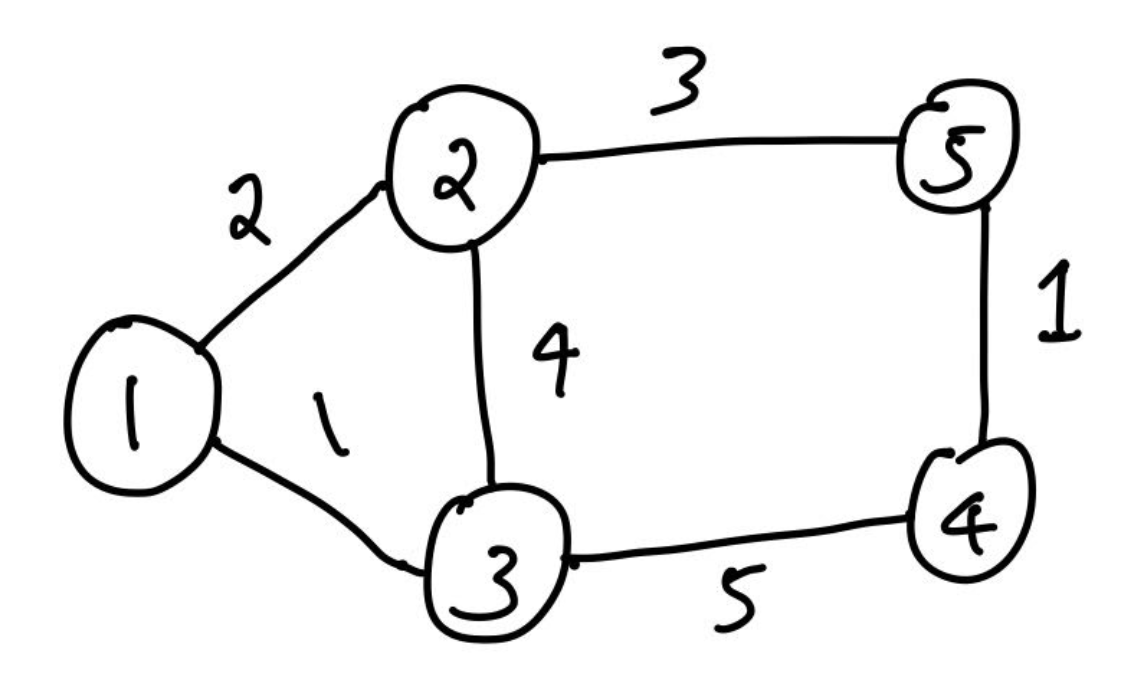
\includegraphics[scale=0.3]{eg1}
\end{minipage}
\hfill
\begin{minipage}{0.5\textwidth}
For $S = \{1,2, 3\}$, $\mathcal{W}(S) = 8$. \\
For $S = \{1,2, 3, 4\}$, $\mathcal{W}(S) = 4$. \\
For $S = \emptyset$, $\mathcal{W}(S) = 0$.
\end{minipage}
\end{figure}
In this example, the maxcut occurs for $S = \{1, 2, 3\}$.
\end{example}

\begin{mdframed}[backgroundcolor=light-gray, linecolor=light-gray]
The decision version (an Yes/No problem) of the maxcut optimization problem is the following
\begin{quote}
{\bf maxcut decision version:} Given a graph and a number $k$, does there exists a cut of weight at least $k$?
\end{quote}
It is known that the problem is \NP-complete. It is easy to see that the problem is in \NP. Just guess the cut $S$ and verify its weight is at least $k$. We skip the proof of hardness. 

It is also easy to see that if we can solve the optimization problem in polynomial time, then the decision version is in \Ptime. What about the other direction: Can we solve the optimization problem in polynomial time if the decision version is in \Ptime? Here is a first attempt. Run the decision version for the weight $k$ ranging from $0$ to $W$ (sum of all weights). The largest $k$ which returns Yes to the decision problem is the weight of maxcut. To find the maxcut from this $k$, we can do the following. Pick an edge $(i,j)$ and force this edge to be in the maxcut by giving it a weight of $W+w_{ij}$. If this edge was in the original maxcut the decision version should return Yes for the new graph and weight $W+k$; otherwise, it should return No. Once the decision on edge $(i,j)$ is made, pick another edge and repeat the procedure (with a slight change). If the previous edge was in the maxcut, update the weight of that edge to $W+w_{ij}$ and continue; if the edge was not in maxcut we go back to our original graph. This procedure is repeated at most $m$ times where $m$ is the number of edges. The total running time is, therefore, a polynomial times $W$. This algorithm runs in pseudo-polynomial time since $W$ is ``exponential in the input size'' because the numbers used to represent weights are represented in binary. We need to get this running time down to $\log W$. In the second attempt, we do a binary search from $0$ to $W$. We run the decision version with $k=\frac{W}{2}$ and based on whether the answer is Yes or No, we search the range $[0, W/2]$ or $[W/2, W]$. 

In short, the optimization and decision versions are ``similar'' in their running time. Given that the decision problem is \NP-hard, there is little hope of a polynomial-time algorithm for the optimization version. 
\end{mdframed}
\notess{Can we simplify the argument on equivalence of decision and optimization version}

It is improbable that maxcut can be solved in polynomial time. What can we hope for? In many practical applications, an ``approximate'' to the best solution is better than no solution. Does there exist a polynomial-time algorithm that can approximate the maxcut? Before we answer that, we need to define the meaning of an approximate solution. For an input graph $G$, we denote by $\opt(G)$ the weight associated with the maxcut. That is, 
\[
\opt(G) \defs \max \{\mathcal{W}(S) \mid S \text{ is a subset of vertices in } G \}
\]
The aim of an approximation algorithm is to find a cut whose weight is very near to $\opt(G)$. Let us assume you have written such an approximation algorithm \A. Clearly, 
\[
\A(G) \leq \opt(G)
\]
We say that algorithm \A\ is an $\alpha$-approximation for an $\alpha \in (0,1]$ if 
\[
\alpha ~\opt(G) \leq \A(G), \tag{ for all input instance $G$}
\]
The larger the $\alpha$ is, the better the approximation algorithm is. Our aim is to show that maxcut has a $\approxratio$-approximation. That is, we give an algorithm \A\ such that
\[
\approxratio ~\opt(G) \leq \A(G) \leq \opt(G), \tag{for all input instance $G$}
\]
Can we do better than this? What about a $0.999$-approximation?  This is unforunately not possible. The result follows from a deep result known as the PCP-theorem (see Arora and Barat complexity theory book \cite{arora}). The theorem, shows that unless \NP=\Ptime, optimization problems like the maxcut problem do not have an $\epsilon$-approximation for all $\epsilon < 1$. Hastad in \cite{hastad} gives an explicit $\epsilon = \frac{16}{17} \approx 0.941$ and shows that any algorithm bettering this $\epsilon$-approximation is not possible. Such problems which admit a ``hardness of approximation'' are said to be \NPX-hard.

Some of you might be wondering if all optimization problems are \NPX-hard. This is not so. The Knapsack problem can be approximated to any $\epsilon$ as one wishes. Such problems are said to admit a PTAS.

\section{Approximate solution to maxcut problem}
Our aim is to give a $\approxratio$-approximation algorithm given in \cite{goemans1}. We relax this condition and give a randomized algorithm. A randomized algorithm takes as input a graph and a sequence of random bits. Let \A\ be a randomized approximation algorithm for maxcut. We are interested in showing the following.
\[
\approxratio ~\opt(G) \leq \Exp{\A(G)} \leq \opt(G), \tag{for all input instance $G$}
\]
where $\Exp{\A(G)}$ is the expectation taken over all the random choices of \A. The algorithm we give uses semi-definite programming. Let us first recast the maxcut problem in similar terms. 
\begin{align}
\max ~\frac{1}{4} \sum_{i \in V} \sum_{j \in V} w_{ij} (1-x_ix_j) \\
\text{ subject to the constraints, } x_i \in \{-1,+1\}  \nonumber 
\end{align}
This is highly non-convex (infact an integer programming problem). For what assignment to $x_i$s do we get the maximum for the objective function? Let $S$ be the maxcut solution. Assign $x_i=1$ if $i \in S$. Otherwise assign $x_i = -1$. Therefore $(1-x_ix_j) = 0$ if $x_i$ and $x_j$ are both in $S$ or both not in $S$. Otherwise $(1-x_ix_j) = 2$. In short, the weight in the cut $S$ is added twice (since it is multiplied with $2$) whereas the weights outside the cut are not added. Thus, a maxcut solution produces the optimum solution to the above problem. How about the other direction? Does an optimal solution to the above problem give rise to a maxcut solution? This is left as an exercise.

We slightly modify the above problem and give an equivalent version. 
\begin{align}
\label{p:maxcut}
\max ~\frac{1}{4} \sum_{i \in V} \sum_{j \in V} w_{ij} (1-X_{ij})  \\
\text{ subject to the constraints, } \nonumber \\
X = \vec x \trans{\vec x} \text{, and } \nonumber \\
X_{ii} = 1 \tag{for all $i \in V$}
\end{align}
Here $\trans{ \vec x}$ is the transpose of the vector $\vec x$ and $X$ is a matrix. Why is this problem equivalent to our previous problem? All we did was we replaced a ``vector'' view by a ``matrix'' view. The matrix $X$ is a co-variance matrix of $\vec x$. The entry at $X_{ij} = x_i x_j$ for all $i, j \in V$. The equivalence of the above two problems is left as an exercise.

We now show how to approximate \ref{p:maxcut}. There are three important steps.
\begin{enumerate}
\item Approximate \ref{p:maxcut} by a convex optimization problem \ref{p:sdp}.
\item Decompose the solution to the optimization problem \ref{p:sdp}.
\item Extract a cut set from this decomposition.
\end{enumerate}
We now provide details of each of the steps mentioned above. It is also shown that this approximation algorithm runs in polynomial time. The argument that this is indeed a $\approxratio$-approximation is deferred to the next section.

\paragraph*{Step 1: Approximate \ref{p:maxcut} by a convex optimization problem}
The approximation is by a semi-definite program (SDP). An SDP is a special case of a convex optimization problem. 
\begin{align}
\label{p:sdp}
\max ~\frac{1}{4} \sum_{i \in V} \sum_{j \in V} w_{ij} (1-X_{ij}) \\
\text{ subject to the constraints, } \nonumber \\
X = \Matrix{1, x_{11}, \cdots,x_{1n-1},x_{1n}; x_{11}, 1, \cdots,\cdots ,x_{2n};,\cdots,\cdots,\cdots;x_{1n-1},\cdots,\cdots,1,x_{n-1n};x_{1n},x_{2n},\cdots,x_{n-1n},1 }  \text{ is a psd} \nonumber 
\end{align}
%
The matrix $X$ is a symmetric positive semi-definite matrix (psd). Such matrices satisfy the condition that $X = R \trans R$ for an $m \times k$ real matrix $R$. Note that $X$ in problem \ref{p:maxcut} is also a symmetric psd (it is of the form $\vec x \trans{\vec x}$). How is \ref{p:sdp} different from \ref{p:maxcut}?
\begin{enumerate}
\item $X$ in \ref{p:maxcut} was a rank-1 matrix whereas X in \ref{p:sdp} has no rank restriction.
\item The information contained in individual variables $x_i$s are lost in \ref{p:sdp}. Problem \ref{p:sdp} only has the co-variance matrix and the ``hope'' is to retrieve the vectors $\vec x$ from this co-variance matrix.
\item The $x_i$s in \ref{p:maxcut} can only take $+1$ or $-1$ values (since $x_i x_i = 1$) and hence the co-variance matrix $X$ can only contain $+1$ or $-1$ entries. There is no such restriction forced on $X$ in problem \ref{p:sdp}.
\end{enumerate}
%
We have lost quite a lot of information by this relaxation on the matrix $X$. What have we gained? An SDP can be solved in polynomial time even in the worst case. In contrast, the problem \ref{p:maxcut} cannot be solved in polynomial time (unless \Ptime=\NP).
\begin{theorem}
\label{thm:sdp}
There is an algorithm (we call it SolveSDP) that takes as input an SDP \ref{p:sdp} and in polynomial time returns the optimal solution matrix $X$.
\end{theorem}
%
\begin{mdframed}[backgroundcolor=light-gray, linecolor=light-gray]
A caveat: There is a small catch when we say SDP can be solved in polynomial time. The optimal solution $X$ might contain irrational numbers. From an algorithmic point of view, we cannot store or do real number computations. One can work with ``rational numbers'' close to real numbers. We say that matrices $X$ and $Y$ are $\delta$ close if $|X_{ij} - Y_{ij}| \leq \delta$. In other words all the entries are within $\delta$ distance. \\

\noindent {\bf Theorem \ref{thm:sdp}.}
\emph{There is an algorithm, which when given SDP \ref{p:sdp} and a $\delta > 0$, returns a matrix $X$ in time polynomial in the input SDP and $\log 1/\delta$ such that $X$ is $\delta$ close to the optimal solution. }

\emph{Moreover, $X$ is a symmetric psd.}\\

Note that the algorithm can get very close to the optimal value. How close, is based on the parameter $\delta$. The closer to the optimal value of the SDP, the more the running time.
\end{mdframed}

\paragraph*{Step 2: Decomposing the matrix $X$}
Our aim is to now extract the cut set from the solution $X$ of \ref{p:sdp}. In Problem \ref{p:maxcut}, $X$ is of the form $\vec x \trans{\vec x}$. The binary value of $x_i$ decides whether the vertex $i$ is in the maxcut or not. Unfortunately, the matrix $X$ of \ref{p:sdp} need not be of this form. 
%

Let us consider the $X$ of \ref{p:sdp}. Since $X$ is symmetric and psd, we can decompose the matrix into a product of a matrix and its transpose. That is, there exists an $n \times k$ real matrix $U$ such that $X = U \trans{U}$. \notess{We want all rows to be distinct if later $X_{ij} \neq 1$. Can we assume that?}
\begin{lemma}[Cholesky decomposition]
\label{lem:cholesky}
There is an $O(n^3)$ algorithm which on input a symmetric psd $X$ returns a matrix $U$ such that $X = U \trans{U}$. 
\end{lemma}
\begin{proof}[Proof sketch.]
The proof of the decomposition involves basic linear algebra. We give a short sketch of the proof. Any full ranked symmetric matrix can be decomposed into the form $L D \trans L$ where $L$ is a lower triangular matrix and $D$ is a diagonal matrix. Standard Guassian elimination can achieve this in $O(n^3)$ time. Since a psd has non-negative pivots (follows from the fact that eigen values of psd are non-negative), the diagonal matrix $D$ can be written as the product of two ``square root'' matrices. This concludes the proof.
\[X = LD \trans L = L \sqrt D \sqrt D \trans L = L \sqrt D \trans{(\sqrt D L)} = U \trans U \]
A detailed argument can be found in Section \ref{sec:cholesky}.
\end{proof}
The row vectors $\vec u_i$s of $U$ are important for us. Since the diagonal elements $X_{ii}$ are equal to $1$, the vectors $\vec u_i$s have norm $1$.
\[ 
X_{ii} = \trans{\vec{u_i}} \vec{u_i} = 1 \tag{for all row vectors $u_i$ of $U$}
\]


\begin{mdframed}[backgroundcolor=light-gray, linecolor=light-gray]
A caveat: Again there is a problem when the decomposition matrix $U$ is irrational. This is highly likely since as we explained above $U$ is a product of a 
square root matrix. We have to go for an approximate decomposition of a symmetric psd. \\

\noindent {\bf Lemma \ref{lem:cholesky}} (Cholesky decomposition). 
There is a real matrix $U$ such that $X = U \trans{U}$. Moreover, there is an algorithm, which given $X$ and a $\delta > 0$, returns $U$ in time polynomial in input size of $X$ and $\log 1/\delta$ such that
\[
\widehat X_{ij} -\delta \leq X_{ij} \leq  \widehat X_{ij} + \delta
\]
where $\widehat X = U \trans{U}$. In short, $\widehat X$ is $\delta$ close to $X$. \\

\noindent The diagonal elements in $X$ are $1$ and therefore the diagonal elements in $\widehat X$ are close to $1$. Therefore
\[
1 -\delta \leq \trans{\vec{u_i}} \vec{u_i} \leq  1 + \delta \tag{for all row vectors $u_i$ of $U$}
\]
\end{mdframed}

\paragraph*{Step 3: Extracting a cut set from the decomposition matrix $U$:}
The row vectors of $U$ (denoted as $\vec u_i$s) help us identify a cut $S$. Recap how $x_i$s in Problem \ref{p:maxcut} (the original maxcut problem) determined whether $i$ is in the maxcut or not. In that setting, vertices $i$ and $j$ fall in the same set (either $S$ or $T$) if $x_i=x_j$. The reason is that $(1-x_ix_j)$ is zero when this happens, and therefore these vertices are not contributing to the optimization function. On the other hand, if $x_i \neq x_j$ we require them to be in different sets since $(1-x_ix_j) =2$ and therefore are contributing to the optimization function. Let us return to the problem \ref{p:sdp} and the vectors $\vec u_i$ and $\vec u_j$. We have that $X_{ij} = \trans{\vec u_i} \vec u_j$. When $X_{ij}$ is high (close to $1$) we should ideally have $i$ and $j$ in the same set. Since the inner product is proportional to the angle between the vectors, it follows that we want $i$ and $j$ to be in the same set if the angle between $\vec u_i$ and $\vec u_j$ is small. There is a problem, however. The angle between vectors $\vec u_i$ and $\vec u_j$ can be small, and that between $\vec u_j$ and $\vec u_k$ is small, but the angle between $\vec u_i$ and $\vec u_k$ is not small. We are in a predicament whether to include all the three vectors $i, j$ and $k$ in the same set or not. The angle between the vectors is not an ``equivalence'' relation. Therefore, we are interested in a ``clustering'' algorithm - partition the vectors $\vec u_i$s into two parts such that angles inside a part are minimized. \notess{The original problem is a clustering problem on graphs. We have reduced it to a clustering problem on vectors. Why does this help?}

The problem is resolved using randomization. We pick a random vector $\vec r$ and all vectors close to it (less than $90$ degree) are included in $S$ whereas all other vectors are in $T$. 
It is easy to observe that the algorithm runs in randomized polynomial time. \Cref{alg:cluster} gives the details.  
\begin{algorithm}[h!]
\caption{Cluster the vectors into two parts}
\label{alg:cluster}
\begin{algorithmic}
\STATE Initialize set $S = \emptyset$.
\STATE Pick a random vector $\vec r \in \Reals^{|V|}$ such that $|\vec r|_2 = 1$.	 
\FOR {$i \in V$}
	\IF {$\trans{\vec r} \vec{u_i} \geq 0$}
		\STATE add $i$ to $S$
	\ENDIF
	\STATE \comment{$i$ is not added to $S$ if $\trans{\vec r} \vec{u_i} < 0$}
\ENDFOR
\RETURN $S$
\end{algorithmic}
\end{algorithm}
\notess{Why suddenly randomization comes in for clustering?}
\notess{Why do we want $|\vec r|=1$?}

\begin{mdframed}[backgroundcolor=light-gray, linecolor=light-gray]
In the above algorithm, the only non-trivial part is picking a random vector $\vec r$ in the unit sphere's surface. We can do this by picking $r_i$ randomly from the normal distribution $\mathcal{N}(0,1)$. With a high probability, $\vec r$ is in the unit sphere's surface; the probability increases with the dimension. There are some implementation issues. Theoretically, we pick real numbers from the normal distribution. But practically, we leave out all the real numbers. Moreover, the rational numbers we pick can only be of the form $\frac{p}{q}$ where $p$ and $q$ are polynomial in the size of the input. Thus, an ``algorithm'' assigns all ``un-representable'' numbers to probability $0$. Does picking from the rest of the numbers (based on normal distribution probability) also give a vector on the surface of the unit sphere? 
\end{mdframed}

This concludes the randomized algorithm. It consists of mainly three steps, each running in polynomial time. $(1)$ Approximation using SDP, $(2)$ Cholesky decomposition of the solution to the SDP $(3)$ Clustering the vectors from the decomposition. In the next section we show that this algorithm gives in expectation a maxcut which is $\approxratio$-approximate.


\begin{mdframed}[backgroundcolor=light-gray, linecolor=light-gray]
Some questions:
\begin{enumerate}
\item Rather than pick a random vector $\vec r$, why do we not pick one of the vectors $\vec u_i$ randomly, and add all $\vec u_j$s close to it into $S$.
\item Is there any relation between rank of returned $X$ and the closeness of approximation? We know that if rank is $1$ then we will get the optimal solution to maxcut.
\item Why not do the following. Let SDP return matrix $X$. We find the best 1-rank approximation to $X$ and use that as indicator for recognizing the cut. Finding the best 1-rank approximation can be done in polytime (I guess so??) - only required to find the largest singular value and left and right singular vectors.
\end{enumerate}
\end{mdframed}


\section{Establishing the Approximation ratio}
Let us recall the Algorithm for approximating maxcut (see \cref{alg:maxcut}). We call this algorithm \A. Let us assume \A\ returns $S$ on input $G$.

\begin{algorithm}[h!]
\caption{$ApproximateMaxCut$}
\label{alg:maxcut}
\begin{algorithmic}[1]
\STATE \comment{Input: A weighted graph $G=(V,E)$}
\STATE \comment{Output: A $\approxratio$-approximation to maxcut}
\STATE SDP $P =$ Approximate the maxcut problem into the form \ref{p:sdp}
\STATE \comment{Solve the SDP $P$}
\STATE $X$ = SolveSDP$(P)$ 
%\STATE \comment{$X$ is $\delta$ close to the optimal solution to SDP $P$}
\STATE \comment{Decompose $X$ into  $U \trans{U}$}
\STATE $U$ = Cholesky-Decomposition$(X)$ 
%\STATE \comment{$X$ is $\delta$ close to $U \trans{U}$}
\STATE Let $\{u_1, \dots, u_{|V|}\}$ be the rows of $U$.
\STATE Let $S = \emptyset$. \comment{ Set $S$ will be the cut.}
\STATE Pick a random vector $\vec r \in \Reals^{|V|}$ such that $|\vec r|_2 = 1$.	
\FOR {$i \in V$}
	\IF {$\trans{\vec r} \vec{u_i} \geq 0$} 
		\STATE \comment{angle between $\vec r$ and $\vec u_i$ is less than $90$ degree}
		\STATE add $i$ to $S$ 
	\ENDIF
	\STATE \comment{$i$ is not added to $S$ if $\trans{\vec r} \vec{u_i} < 0$}
\ENDFOR
\RETURN $S$
\end{algorithmic}
\end{algorithm}

\begin{mdframed}[backgroundcolor=light-gray, linecolor=light-gray]
For analysis, we will assume that SolveSDP and Cholesky-Decomposition gives the optimal matrix $X$ and the exact decomposition matrix $U$ and not a $\delta$ approximation in either of the two cases. 
\end{mdframed}

Our aim is to show that
\[\approxratio ~\opt(G) \leq \Exp {\mathcal{W}(S)} \]
where the expectation is computed over the random choices of $\vec r$. Consider the indicator random variables $Y_{ij}$
\[
Y_{ij} = \begin{cases}
0, \text{ if $i$ and $j$ are either both in $S$ or both in $T$}  \\
1, \text{ otherwise} 
\end{cases}
\]
We can calculate the expected weight of the cut returned by \A.
\begin{align*}
\Exp{\mathcal{W}(S)} & = \Exp{\frac{1}{2} \sum_{i \in V} \sum_{j \in V} \Big(w_{ij} ~Y_{ij} \Big) } \\
& = \frac{1}{2} \sum_{i \in V} \sum_{j \in V} \Big(w_{ij} ~\Exp{Y_{ij}} \Big) \tag{ by linearity of expectation} \\
& = \frac{1}{2} \sum_{i \in V} \sum_{j \in V} \Big(w_{ij} (1-X_{ij}) ~\frac{\Exp{Y_{ij}}}{1-X_{ij}} \Big) 
 = \frac{1}{4} \sum_{i \in V} \sum_{j \in V} \Big(w_{ij} (1-X_{ij}) ~\frac{2 ~\Exp{Y_{ij}}}{1-X_{ij}} \Big) \\
& \geq \min_{i,j \in V} \Big\{~\frac{2 ~\Exp{Y_{ij}}}{1-X_{ij}} \Big\} ~\frac{1}{4} \sum_{i \in V} \sum_{j \in V} w_{ij} (1-X_{ij}) \\
& = \min_{i,j \in V} \Big\{\frac{2 ~\Prob{Y_{ij} = 1}}{1-X_{ij}} \Big\} ~\frac{1}{4} \sum_{i \in V} \sum_{j \in V} w_{ij} (1-X_{ij}) \tag{Since $Y_{ij}$ is an indicator random variable} \\
& = \min_{i,j \in V} \Big\{\frac{2 ~\Prob{Y_{ij} = 1}}{1-X_{ij}} \Big\}  ~\opt(G) 
\end{align*} \notess{If $1-X_{ij}=0$ we cannot multiply and divide. What happens if $\vec u_i = \vec u_j$?}
The last equality follows from the fact that $X$ is an optimal solution to \ref{p:sdp} and $\opt(G)$ is achieved by an $1$-rank matrix $\hat X$ which is a feasible solution (and need not be optimal) for the SDP \ref{p:sdp}. 
It is sufficient to bound 
\[ \min_{i,j \in V} \Big\{\frac{2~\Prob{Y_{ij} = 1}}{1-X_{ij}}\Big\} > \approxratio \]

First, we find the probability that $i$ and $j$ are on the opposite sides of the cut. By our algorithm, this happens if and only if the angle between $\vec r$ and $\vec u_i$ is acute and the angle between $\vec r$ and $\vec u_{j}$ is obtuse or vice versa.  
\[
\Prob{Y_{ij} = 1} = 2 ~\Prob{\trans {\vec r} \vec u_i \geq 0 \text{ and } \trans {\vec r} \vec u_j < 0 }
\]
Let $\theta$ be the angle between vectors $\vec u_i$ and $\vec u_j$. We show the following
\[\Prob{\trans {\vec r} \vec u_i \geq 0 \text{ and } \trans {\vec r} \vec u_j < 0 } = \frac{\theta}{2 \pi} \]
This is \emph{rotational symmetric} - the probability remains the same if we rotate all the vectors by the same angle.  
\[\Prob{\trans {\vec r} \vec u_i \geq 0 \text{ and } \trans {\vec r} \vec u_j < 0 } = \Prob{\trans {(Q \vec r)} Q \vec u_i \geq 0 \text{ and } \trans {(Q \vec r)} Q\vec u_j < 0 } \]
where $Q$ is any orthonormal matrix - columns are perpendicular to each other and also have unit norm. Therefore $\trans{Q} Q$ is the identity matrix. Rotational matrices are orthonormal matrices. Let $Q$ be a matrix which rotates $\vec u_i$ to the x-axis (giving $\hat {\vec u_i}$) and $\vec u_j$ to the x-y plane (giving $\hat {\vec u_j}$) . In other words except for the first co-ordinate in $\hat {\vec u_i}$ and the first two co-ordinates in $\hat {\vec u_j}$ all other co-ordinates are zero. That is, $\hat {\vec u_i} = (u_i^1,0, 0, \dots, 0)$ and $\hat {\vec u_j} = (u_j^1, u_j^2, 0, 0, \dots, 0)$. Let $\hat{\vec r}$ be the projection of $\vec r$ on the x-y plane. Since apart from the first two co-ordinates all the other co-ordinates of $\hat {\vec u_i}$ and $\hat{\vec u_j}$ are zeros, $\trans {\vec r} \hat {\vec u_i} = \trans {\hat{\vec r}} \hat {\vec u_i}$ and $\trans {\vec r} \hat {\vec u_j} = \trans {\hat{\vec r}} \hat {\vec u_j}$. So, it is sufficient to analyse the probability in the 2 dimensional x-y plane.

\Cref{fig:angleanalysis} provides a ``visual'' proof of $\Prob{\trans {\vec r} \vec u_i \geq 0 \text{ and } \trans {\vec r} \vec u_j < 0 } = \frac{\theta}{2 \pi}$. 
Hence $\Prob{Y_{ij}=1} = \frac{\theta}{\pi}$. Therefore
\[ 
\frac{2~\Prob{Y_{ij} = 1}}{1-X_{ij}} = \frac{2~\theta}{\pi (1-X_{ij})} = \frac{2~\theta}{\pi (1-\cos \theta)}
\]
The last equality comes from the fact that $X_{ij} = \trans{\vec{u_i}} \vec u_j = \cos \theta$, and because for all $l \in V$, $\trans{\vec u_l} \vec u_l = 1$.
The paper \cite{goemans1} claims that basic calculus shows
\[
\min_{i,j \in V} \Big\{ \frac{2~\theta}{\pi (1-\cos \theta)} \Big\} > \approxratio 
\]
This concludes the proof.
\def\myrad{2cm}% radius of the circle
\def\myang{60}% angle for the arc

\begin{figure}[h!]
\begin{minipage}{0.3\textwidth}
\begin{tikzpicture}
% the origin
\coordinate (O) at (0,0);
% the circle and the dot at the origin
\draw (O) node[circle,inner sep=1.5pt,fill] {} circle [radius=\myrad];
% the ``\theta'' arc
\draw
  (\myrad,0) coordinate (xcoord) -- 
  node[midway,below] {$\vec u_i$} (O) --
  (\myang:\myrad) coordinate (slcoord) 
   node[midway,left] {$\vec u_j$} (O) ;
%  pic [draw,->,angle radius=1cm] {angle = xcoord--O--slcoord};
% the outer ``s'' arc

\draw[red,thick, ->] (0,0) -- (\myrad,0);
\draw[red,thick,dashed] (0,0) -- (0, \myrad);
\draw[red,thick,dashed] (0,0) -- (0, -\myrad);

\draw[blue,thick, ->] (0,0) -- (\myrad * 0.51,\myrad * 0.87);
\draw[blue,thick,dashed] (0,0) -- (\myrad * 0.87,-\myrad * 0.51);
\draw[blue,thick,dashed] (0,0) -- (-\myrad * 0.87,\myrad * 0.6);

\node[draw] at (-0.6,1.2) {A};
\node[draw] at (-0.8,-1) {B};
\node[draw] at (0.6,-1) {C};
\node[draw] at (1.4,1) {D};

\draw (0.5,0) -- (0.5,0.5) -- (0,0.5);

\draw[|-|]
  (1,0)
  arc[start angle=0,end angle=\myang,radius=1]
    node[midway] {$\theta$};

%\draw[|-|]
%  (\myrad * 0.87,-\myrad * 0.51)
%  arc[start angle=-30,end angle=\mynty,radius=\myrad+10pt]
%    node[midway,fill=white] {$s$};
\end{tikzpicture}
\end{minipage}
\hfill
\begin{minipage}{0.55\textwidth}
\begin{enumerate}
\item Region A: $\trans{\vec r} \vec u_i \geq 0$ and $\trans{\vec r} \vec u_j < 0$
\item Region B: $\trans{\vec r} \vec u_i \geq 0$ and $\trans{\vec r} \vec u_j \geq 0$
\item Region C: $\trans{\vec r} \vec u_i < 0$ and $\trans{\vec r} \vec u_j \geq 0$
\item Region D: $\trans{\vec r} \vec u_i < 0$ and $\trans{\vec r} \vec u_j < 0$
\end{enumerate}
\end{minipage}
\caption{A random vector $\vec r$ can lie in any of the four regions. Region A (resp. C) cover $\frac{\theta}{2 \pi}$ of the area. The probability that $i \in S$ and $j \notin S$ is equal to the area of region A.}
\label{fig:angleanalysis}
\end{figure}

\begin{mdframed}[backgroundcolor=light-gray, linecolor=light-gray]
If the matrices have irrational entries, we work with matrices $\delta$ close to the optimal. Maintaining an $\approxratio$-approximation is possible since we can take a $\delta$ as close to the optimal as we want. The argument needs to thought through.
\end{mdframed}

\section{Cholesky decomposition}
\label{sec:cholesky}
In this section our aim is to show that a symmetric positive semi-definite matrix $X$ can be written as a product of a matrix and its transpose. 

\begin{mdframed}[backgroundcolor=light-gray, linecolor=light-gray]
We say a matrix is lower triangular (resp. upper triangular) if all entries above (resp. below) the diagonal are zero and the diagonal entries are $1$.
\begin{claim}
Let $X$ be any full rank matrix. Then $X = L D U$ for a lower triangular matrix $L$, diagonal matrix $D$ and upper triangular matrix $U$. 

Moreover if $X$ is rational $L, D$ and $U$ are rational and an algorithm can output $L, D$ and $U$ in $O(n^3)$.
\end{claim}
\begin{proof}[Proof sketch (see Strang \cite{strang}).] Consider the full rank matrix $X$. We can do a row operation and make the first column second row cell to zero. Let this new matrix be $Y$. You can also go back from $Y$ to $X$ be doing the reverse row operation. Both these row operations (are linear transformations) are equivalent to multiplication by a lower triangular matrix. That is
\[ X = \hat L Y \tag{ where $\hat L$ is lower triangular } \]
By a series of such operations (gaussian elimination) you can get a matrix $\hat U$ where all entries below the diagonal are zero (the diagonal entries need not be $1$). These series of row operations are equivalent to multiplication by lower triangular matrices. Since product of lower triangular matrices are lower triangular we have
\[ X = \hat L_1 \hat L_2 \dots \hat L_n \hat U = L \hat U \tag{ here $L$ is lower triangular} \]
We can factor out the diagonal elements in $\hat U$ as follows
\begin{align*}
\hat U &= \Matrix{d_1, , , ; , d_2, , ;, , \cdot, ;, , , d_n} \Matrix{1, a_{12}/d_1, a_{13}/d_1, ; ,1, a_{23}/d_2, ; , , \cdot, ; , , , 1} \\
&= D ~U \tag{here $D$ is diagonal and $U$ is upper triangular}
\end{align*}
Therefore $X = L D U$. By a careful analysis one can establish that this decomposition can be done in $O(n^3)$.
\end{proof}
\begin{claim}
\label{claim:sym}
Let $X$ be a symmetric full rank matrix. Then $X = L D \trans L$ for a diagonal matrix $D$ and lower triangular matrix $L$. Moreover, if $X$ is rational $L$ and $D$ are rational.
\end{claim}
\begin{proof}
Since $X = LDU$ by the above theorem and $X = \trans{X}$ we have $X = LDU = \trans{U} D \trans{L}$. Take $L$ to the other side. That is $D U (\trans L)^{-1} = L^{-1} \trans{U} D$. Since one is a left triangular matrix and the other right triangular, the only possibility is it is a diagonal matrix. By looking at the diagonals it follows that $L = \trans U$.
\end{proof}
\end{mdframed}

We now show that symmetric psd matrices $X$ have a factorization $V \trans V$.
We make use of the following property of psd matrices.
\begin{lemma}
\label{lem:psd}
$X$ is psd iff the pivots of $X$ are greater than or equal to $0$.
\end{lemma}

\noindent{\bf Lemma \ref{lem:cholesky}} (Choleksy decomposition). 
%A symmetric psd $X=V \trans V$ for a real matrix $V$. 
\emph{Let $\delta > 0$. There is an algorithm, given a symmetric psd $X$ and $\delta$ returns a $V$ in
 time polynomial in input $X$ and $\log 1/\delta$ such that $X$ is $\delta$ close to $V \trans V$.}
\begin{proof}
Let us assume $X$ is a full rank symmetric psd. Since $X$ is symmetric and full rank we have that $X = LD \trans L$ from \cref{claim:sym}. From previous claim the pivots are non-negative and therefore $D$ does not contain any negative numbers. Hence a square root of $D$ is possible.
\[
X = LD \trans L = L \sqrt D \sqrt D \trans L = L \sqrt D \trans{(\sqrt D L)} = V \trans V
\]
It is clear that the only place where approximation is required is to find the square root of the diagonal entries. Newton's method (??) can approximate this to an accuracy as claimed in the statement of the theorem.

We have to finally, consider the case of a symmetric psd that is not full rank. We leave this as an exercise to the reader. 
\end{proof} 

\bibliography{papers}
\bibliographystyle{plain}
\end{document}
